\documentclass[11pt,article]{amsart}

%----------Packages----------
\usepackage{amsmath} %%Mathpackage
\usepackage{amssymb} %%Mathpackage
\usepackage{amsthm} %%Mathpackage
\usepackage{dsfont}
\usepackage{mathrsfs}
\usepackage{stmaryrd}
\usepackage{enumerate} %%To use the enumerate environment
\usepackage{verbatim} %%Shows the text as typed
\usepackage{fullpage}  %%smaller margins
\usepackage{multicol}
\usepackage{tikz}
\usepackage{url}
\usetikzlibrary{arrows.meta}

%----------Theorems----------

\newtheorem{theorem}{Theorem}[section]
\newtheorem{proposition}[theorem]{Proposition}
\newtheorem{lemma}[theorem]{Lemma}
\newtheorem{corollary}[theorem]{Corollary}
\newtheorem{axiom}{Axiom}
\newtheorem*{theorem*}{Theorem}


\theoremstyle{definition}
\newtheorem{definition}[theorem]{Definition}
\newtheorem{nondefinition}[theorem]{Non-Definition}
\newtheorem{exercise}[theorem]{Exercise}
\newtheorem{remark}[theorem]{Remark}
\newtheorem{warning}[theorem]{Warning}
\newtheorem*{goal}{Goal}

%----------Commands----------
\newcommand\tab[1][1cm]{\hspace*{#1}}
%https://tex.stackexchange.com/questions/198432/using-the-tab-command

\numberwithin{equation}{subsection}

%\documentclass[titlepage]{article}
\author{Ross Blassingame, Michael Tang}
\title{An Analysis on List Allocation on the Stack through Escape Analysis}
\begin{document}
\maketitle
\begin{multicols}{2}
\section{abstract}
This analysis presents a simple escape analysis algorithm to determine (i) which variables outlive its scope, and subsequently, (ii) which variables that are lists, will be stack allocable, reducing list allocations on the heap. This algorithm takes inspiration from escape analysis found in Java, which determine objects that are stack allocable in methods. A $Connection$ $Graph$ will be utilized to represent connections between lists and references to lists during the analysis to determine escaping variables. 
\section{Introduction}
Our Python compiler depends upon the C runtime library for current heap-allocated objects. The responsibility of memory management belongs to the C runtime to release, $free$, heap allocated- resources. In an ideal environment, heap-allocated resources should be released; otherwise, (1) memory leak will occur. (2) The latency of heap usage arise within the generated assembly code, which calls the runtime C function for object creation and subscription, $in$ $terms$ $of$ $lists$. From escape analysis, we will be able to determine which variables escape its scope and which variables remain local to its scope $(non$-$escaping)$. Once determined, variables that are lists and non-escaping can be stack allocatable. Stack allocation removes the risks in (1) \& (2). 

\section{Notation}
We define some mathematical notation to aid our analysis. 
\begin{definition}
Let $v$ be a variable defined in a scope $S$. We say $v$ escapes $S$ if the lifetime of $v$ outlives $S$, denoted $Escape(v,S)$.
\end{definition}
3.1 describes a scenario where a variable $v$, defined in some scope, is escaping when its usage is existent after the scope no longer exists.  
\begin{definition}
Let $v$ be a variable that is defined or referenced in a scope $S$. Then $\forall v\in S$, we say that $v$ will either be in one of the three sets: $NoEscape$, $ArgumentEscape$, $GlobalEscape$ i.e. $(v\in NE \oplus v\in AE \oplus v\in GE)$ != $(v\in NE \wedge v\in AE \wedge v\in GE)$. 
\end{definition}
The following definitions describe these sets.  
\begin{definition}
$v\in NE$ if for some scope $S$, $\neg Escape(v,S)$.
\end{definition}
\begin{definition}
$v\in AE$ for some function's scope $S_f$ if for some function argument $a$ that belongs to $f$ is an object having attribute $x$, then $\exists a.x = v \in S_f$. We also say that $Escape(v, S_f)$ and $Escape(a.x, S_f)$.
\end{definition}
The definition of $AE$ says that if an object $a$ with attribute $x$ is passed as an argument to some function $f$ and there exists assignment statements of the form $a.x = v$, then we classify $a.x$ and $v$ as escaping. 
\begin{definition}
$v\in GE$ for some function's scope $S_f$ if for some $p \in OuterScopeVariable$, $\exists p = v \in S_f$. We say $Escape(v, S_f)$ and $Escape(p, S_f)$. For some class $C \notin S_f$, if $\exists C.x = v \in S_f$, then $Escape(v, S_f)$ and $Escape(C.x, S_f)$
\end{definition}
The definition of $GE$ says if a variable $p$ that is outside of the current scope, assignments within the scope to $p$ will cause it to be escaping and whatever it was assigned to be escaping as well. The second half of the definition talks about static class fields. We first put a constraint on behavior of the class $C$ not being in the scope of $S_f$. The reason for is because a class may be defined within a function, and if all instantiations of the class within the function remain non-escaping along with the class itself, then there is no reason to mark $C.x$ or $v$ as escaping. If this is not the case, then both $C.x$ and $v$ will be escaping. 

\begin{definition}
A $Connection$ $Graph$ is a directed graph where node within the graph are composed of variables $v \in NE \cup AE \cup GE$, list objects, and $return$ node(s). Edges within the graph show assignments. We denote $v \xrightarrow[]{\text{P}} l$, where the $P$ is a $point$-$to$ $path$ edge, and we denote $v \xrightarrow[]{\text{D}} v_1$, where $D$ is a $deferred$ $edge$
\end{definition}
Clarifying on 3.6, a connection graph is made up of nodes that represent a given scope. Nodes are composed of variables, lists, primitives, and return statements. We specify return statements as its own node in the connection graph since it serves a special purpose on figuring out what escapes by what its edge points to in the graph. All return nodes in a connection graph are initially marked to be globally escaping, and we will speak more as to why in section four. Edges are directed in a connection graph, and for our paper, we will condense them to be $point$-$to$ $path$ or $deferred$. A point-to path edge describes the scenario that a variable is assigned directly to a value, and on the graph it takes one-step from said variable node to the value node. A deferred edge describes the case where a variable $v$ is assigned to another variable $v_1$. It may be the case that the graph describes a chain of variable assignments, $v_i$ defined in a scope $S$ i.e. $v \xrightarrow[]{\text{D}} v_1 \xrightarrow[]{\text{D}} v_2 \xrightarrow[]{\text{D}} ... \xrightarrow[]{\text{D}} v_n \xrightarrow[]{\text{P}} l$ where $l$ terminates the chain since it's a list object. Or instead, .$.. \xrightarrow[]{\text{D}} v_n \xrightarrow[]{\text{P}} g$, where $g\in AE \cup GE$.

\begin{definition}
Let $l$ be a list defined within a scope $S$ and $CG$ be a $connection$ $graph$ that describes $S$. By definition 3.6, $NE \subseteq CG$. If $l \in NE$, then $l$ is stack allocable in $S$. If $l \notin NE$, then $l$ must be heap allocated. 
\end{definition}
3.7 gives a restriction on the condition on when a list may be stack allocated. If $l \in NE$, then it means that $l$ does not outlive the scope $S$. This means $l$ can be located on the stack without fear when the stack frame collapses that no references of $l$ exists outside of $S$. Otherwise, $l$ must be heap allocated if $l \notin NE$ since references may exists beyond the lifetime of the stack frame. The worry here is that accessing a stack-allocated list that escapes after the stack frame collapses leads to undefined-behavior. 
\section{Building the Connection Graph}
For our analysis, we will assume that all statements within a scope are flatten. We initially let $CG = \varnothing$; then we append nodes to the graph under the following rules. If a given variable node already exists in $CG$, we replace its outgoing edges with the new node's edges. 
\subsection{p = [...]}
A new list is created, and it's assigned to a variable $p$. We add a new node $p$ to the graph with a point-to path edge $\xrightarrow[]{\text{P}}$ to a new list node $l_0$. 

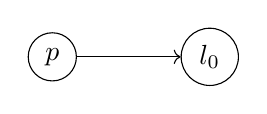
\begin{tikzpicture}
    \node[shape=circle,draw=black] (p) at (1,3) {$p$};
    \node[shape=circle,draw=black] (l) at (3,3) {${l_0}$};
    \path [->] (p) edge node[left] {} (l);
\end{tikzpicture}

$figure.1$ $CG$ after $p$ is assigned to a new list $l_0$.

\subsection{q = p}
We have a variable $q$ that is assigned to the variable $p$. Building along the previous graph, the new graph will have a new node $q$ that has a deferred edge $\xrightarrow[]{\text{D}}$  to $p$.  

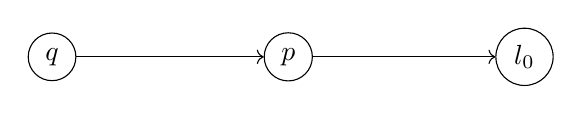
\begin{tikzpicture}
    \node[shape=circle,draw=black] (p) at (3,3) {$p$};
     \node[shape=circle,draw=black] (q) at (0,3) {$q$};
    \node[shape=circle,draw=black] (l) at (6,3) {${l_0}$};
    \path [->] (p) edge node[left] {} (l);
      \path [->] (q) edge node[left] {} (p);
\end{tikzpicture}

$figure.2$ $CG$ after $q$ is assigned to $p$.

\subsection{o.x = p}
We have an object $o$ with attribute $x$ that is assigned to the variable $p$. The new graph will have two new nodes $o \xrightarrow[]{\text{D}} o_x$ where $o_x \xrightarrow[]{\text{D}} p$.  

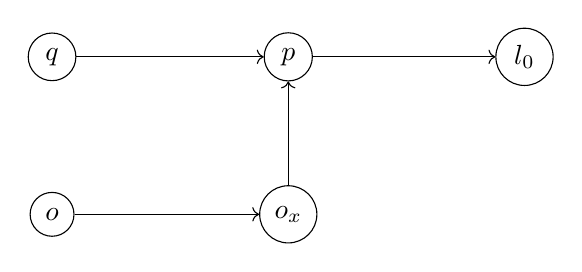
\begin{tikzpicture}
    \node[shape=circle,draw=black] (p) at (3,3) {$p$};
     \node[shape=circle,draw=black] (q) at (0,3) {$q$};
      \node[shape=circle,draw=black] (o) at (0,1) {$o$};
       \node[shape=circle,draw=black] (x) at (3,1) {$o_x$};
    \node[shape=circle,draw=black] (l) at (6,3) {${l_0}$};
    \path [->] (p) edge node[left] {} (l);
    \path [->] (q) edge node[left] {} (p);
    \path [->] (o) edge node[left] {} (x);
    \path [->] (x) edge node[left] {} (p);
\end{tikzpicture}

$figure.3$ $CG$ after $o.x$ is assigned to $p$.

\subsection{s = o.x}
We have an object $o$ with attribute $x$ that variable $s$ is assigned. The new graph will have two new nodes, if $o$ does not already exist, $s \xrightarrow[]{\text{D}} o$ where $o \xrightarrow[]{\text{D}} o.x$.  

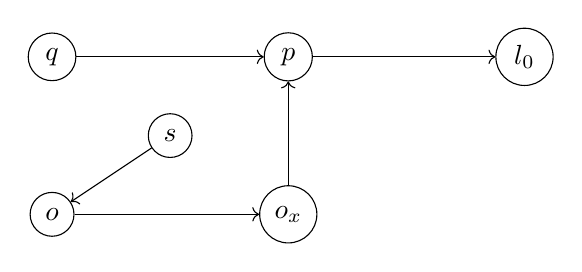
\begin{tikzpicture}
    \node[shape=circle,draw=black] (p) at (3,3) {$p$};
     \node[shape=circle,draw=black] (q) at (0,3) {$q$};
      \node[shape=circle,draw=black] (o) at (0,1) {$o$};
       \node[shape=circle,draw=black] (x) at (3,1) {$o_x$};
    \node[shape=circle,draw=black] (l) at (6,3) {${l_0}$};
    \node[shape=circle,draw=black] (s) at (1.5,2) {$s$};
    \path [->] (p) edge node[left] {} (l);
    \path [->] (q) edge node[left] {} (p);
    \path [->] (o) edge node[left] {} (x);
    \path [->] (x) edge node[left] {} (p);
    \path [->] (s) edge node[left] {} (o);
\end{tikzpicture}

$figure.4$ $CG$ after $s$ is assigned to $o.x$.

\subsection{return q}
We have a return statement that returns the variable $q$. A return statement is a node that is marked as $GE$. $\forall n\in CG$, if there exists a path from $return$ to $n$, then we also mark $n$ as $GE$. \textit{Due to formatting of the graph size, we will abbreviate the node \textbf{return} as \textbf{r} and $GE$ as $\Gamma$}.

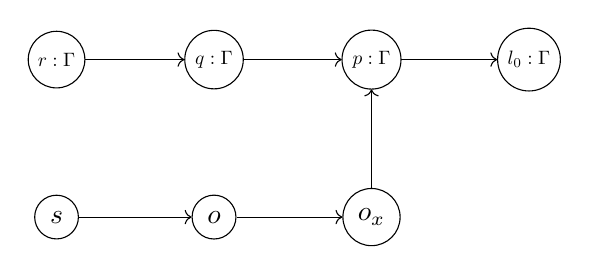
\begin{tikzpicture}
    \node[shape=circle,draw=black,scale=0.7] (p) at (4,3) {$p:\Gamma$};
    \node[shape=circle,draw=black,scale=0.7] (rtn) at (0,3) {$r:\Gamma$};
     \node[shape=circle,draw=black,scale=0.7] (q) at (2,3) {$q:\Gamma$};
      \node[shape=circle,draw=black] (o) at (2,1) {$o$};
       \node[shape=circle,draw=black] (x) at (4,1) {$o_x$};
    \node[shape=circle,draw=black,scale=0.7] (l) at (6,3) {${l_0:\Gamma}$};
    \node[shape=circle,draw=black] (s) at (0,1) {$s$};
    \path [->] (p) edge node[left] {} (l);
     \path [->] (rtn) edge node[left] {} (q);
    \path [->] (q) edge node[left] {} (p);
    \path [->] (o) edge node[left] {} (x);
    \path [->] (x) edge node[left] {} (p);
    \path [->] (s) edge node[left] {} (o);
\end{tikzpicture}

$figure.5$ $CG$ after $q$ is returned. 

\subsection{Remarks to Connection Graph Construction}
In $figure.5$, we hypothetically described the Python program below, assuming that $o$ has already be defined elsewhere:\\
\texttt{p = [1,2,3]}\\
\texttt{q = p}\\
\texttt{o.x = p}\\
\texttt{s = o.x}\\
\texttt{return q}\\
We stated that a return node is marked as $GE$ and that all nodes that can be reached will also be marked as $GE$. Once marking is completed, we have determined which variables can be stack allocated. From $figure.5$, we see that $q$ must be heap allocated by definition 3.7. If we were to modify the code example above to be:\\
\texttt{p = [1,2,3]}\\
\texttt{q = p}\\
\texttt{o.x = p}\\
\texttt{s = o.x}\\
\texttt{return 1.618}\\
The graph will result in looking like:\\
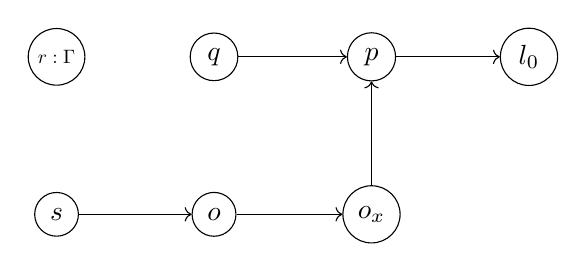
\begin{tikzpicture}
    \node[shape=circle,draw=black] (p) at (4,3) {$p$};
    \node[shape=circle,draw=black,scale=0.7] (rtn) at (0,3) {$r:\Gamma$};
     \node[shape=circle,draw=black] (q) at (2,3) {$q$};
      \node[shape=circle,draw=black] (o) at (2,1) {$o$};
       \node[shape=circle,draw=black] (x) at (4,1) {$o_x$};
    \node[shape=circle,draw=black,] (l) at (6,3) {${l_0}$};
    \node[shape=circle,draw=black] (s) at (0,1) {$s$};
    \path [->] (p) edge node[left] {} (l);

    \path [->] (q) edge node[left] {} (p);
    \path [->] (o) edge node[left] {} (x);
    \path [->] (x) edge node[left] {} (p);
    \path [->] (s) edge node[left] {} (o);
\end{tikzpicture}

$figure.6$ $CG$ stack allocated list.\\ 
We notice that $r:\Gamma$ node is disjoint in the $CG$ graph. Any node that is not marked can be implied that it is non-escaping or $NE$. We can deduce that the list $[1,2,3]$ can be stack allocated, again by definition 3.7.

\subsection{Argument Escape under Connection Graph}
A subtle change happens if we move the code from the previous example into a function, where $o$ is an object. \\
\texttt{def f(o):}\\
\tab\texttt{p = [1,2,3]}\\
\tab\texttt{q = p}\\
\tab\texttt{o.x = p}\\
\tab\texttt{s = o.x}\\
\tab\texttt{return 1.618}\\

Though the return statement is not directly returning back the list $p$, the argument $o$ sets its attribute $x$ to hold $p$, so there is a pathway from $o$ to $p$. By definition 3.4, we can mark $o_x$ and $p$ as escaping from line three within the function. We use $\alpha$ as the marking to show $ArgumentEscape$. And by definition 3.7, after the graph has been marked shows $l_0$ needing to be heap allocated.
%Escape Analysis for Java. Choi J, Gupta M, Serrano M, Sreedhar V, Midkiff S. $https://www.cc.gatech.edu/~harrold/6340/cs6340_fall2009/Readings/choi99escape.pdf$

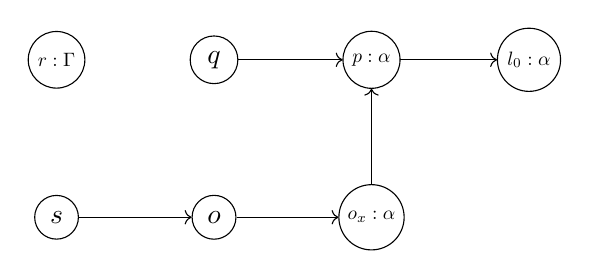
\begin{tikzpicture}
    \node[shape=circle,draw=black,scale=0.7] (p) at (4,3) {$p : \alpha$};
    \node[shape=circle,draw=black,scale=0.7] (rtn) at (0,3) {$r:\Gamma$};
     \node[shape=circle,draw=black] (q) at (2,3) {$q$};
      \node[shape=circle,draw=black] (o) at (2,1) {$o$};
       \node[shape=circle,draw=black,scale=0.7] (x) at (4,1) {$o_x : \alpha$};
    \node[shape=circle,draw=black,scale=0.7] (l) at (6,3) {${l_0 : \alpha}$};
    \node[shape=circle,draw=black] (s) at (0,1) {$s$};
    \path [->] (p) edge node[left] {} (l);

    \path [->] (q) edge node[left] {} (p);
    \path [->] (o) edge node[left] {} (x);
    \path [->] (x) edge node[left] {} (p);
    \path [->] (s) edge node[left] {} (o);
\end{tikzpicture}
$figure.7$ $CG$ on a function showing argument escape.\\ 

\remark{Actions on Stack-
Allocated Lists}
In $P_1$, with the introduction of lists, operations came with that could be applied on lists. Two actions that we will not consider reasonable for the scope of our project is list concatenation and nested lists.  Though these two things are not impossible to optimize in the sense of escape analysis, they present a greater difficulty to implement, so we will avoid these actions on lists and if such occur within a program and heap allocate the result.

\section{Implementation on $P_3$}
For our implementation of stack lists, we map the elements in the list to a 4-byte memory cells where all these memory cells are contiguous on the stack. In addition, we reserve an additional four byte in front of the contiguous memory block. We use this front four bytes to represent the size of the list. All stack lists will have their own first four bytes to represent its size; we abbreviate this memory piece as LSB, $list$ $size$ $byte$. For explication, we need a way to identify at runtime that we are handling a stack-allocated list. For this, we $borrow$ the unused \texttt{0x2} tag, originally reserved for floating-point values, and use it to represent stack lists. In the example Python program below, we represent 4 byte memory cells on the stack as boxes with $v:\epsilon$, where $v$ is either an x86 value or pointer and $\epsilon$ the tag value for $v$, conforming to all $P_1$ tag value besides \texttt{0x2}. \\ \\
\texttt{l = [42,True,False]} \\
$figure.8$ Stack list example program showing implementation.\\ \\
\fbox{$3:0x2$}\fbox{$42:0x0$}\fbox{1:$0x1$}\fbox{0$:0x1$}
$figure.9$ Memory representation layout of figure 8. The left-most block contains the value 3, which represents the size of the list, followed by each element in the list and its tag value. 

\subsection{x86 representation}
We generate the partial x86 code for figure 8. \\
\texttt{.globl main}\\
\texttt{main:} \\
\tab\texttt{pushl \%ebp} \\
\tab\texttt{movl \%esp, \%ebp} \\
\tab\texttt{subl \$20, \%esp} \\
\tab\texttt{movl \$3, \%eax} \\
\tab\texttt{shl \$2, \%eax} \\
\tab\texttt{orl \$2, \%eax} \\
\tab\texttt{movl \%eax, -4(\%ebp)} \\
\tab\texttt{movl \$42, \%eax} \\
\tab\texttt{shl \$2, \%eax} \\
\tab\texttt{orl \$0, \%eax} \\
\tab\texttt{...} \\
\tab\texttt{leal -4(\%ebp), \%eax} \\
\tab\texttt{movl \%eax, -20(\%ebp)} \\
\tab\texttt{addl \$20, \%esp} \\
\tab\texttt{...}\\
$figure.10$ Partial x86 code for figure 8. \\

The x86 code in figure 10 show the stack frame as 20 bytes. The first four bytes being the memory cell that represents the size of the list, followed by three four-byte cells for the elements in the list, and then one four-byte memory region for the variable \texttt{l}. Notice we use the load effective address instruction to retrieve the pointer of the LSB cell and assign it to \texttt{l}.

\subsection{Modifications to the Runtime Library - Printing}
Now that we have stack lists, we need a way for the runtime library to print out this new form of list. We append to the \texttt{runtime.h} and \texttt{runtime.c} the following function prototypes and definitions to allow us to print stack-allocated lists. \\ \\
\texttt{void print\_stack\_list(int* l)\{}\\
\tab\texttt{printf("[");}\\
\tab\texttt{int* ptr = (int*)l;}\\
\tab\texttt{int len = ((*ptr)>>2)-1;}\\
\tab\texttt{ptr--;}\\
\tab\texttt{for(int i = 0; i<len; i++)\{}\\
\tab\tab\texttt{int myPyobj = *ptr;}\\
\tab\tab\texttt{print\_pyobj(myPyobj);}\\
\tab\tab\texttt{printf(", ");}\\
\tab\tab\texttt{ptr--;}\\
\tab\texttt{\}}\\
\tab\texttt{print\_pyobj(*ptr);}\\
\tab\texttt{printf("]\textbackslash n");}\\
\texttt{\}}\\
$figure.11$ Print function for stack-allocated lists. \\    
Building on the example from figure 8,9,10, to call this function in x86, we push the pointer of the LSB of the list. \\
\tab\texttt{movl -20(\%ebp), \%eax} \\
\tab\texttt{pushl \%eax} \\
\tab\texttt{call print\_stack\_list} \\

\section{Conclusion}
Through escape analysis, we can determine what variables escape its scope through the usage of a connection graph. And through an LSB implementation, we can easily modify our current $P_3$ compiler to handle this analysis. Escape analysis reduces unnecessary allocation of heap memory when applicable, conserving heap resources. 

\end{multicols}
\textbf{References:} 
Escape Analysis for Java;  Choi, J. Gupta, M.  Serrano, S. Sreedhar, V. Midkiff, S.
\url{https://www.cc.gatech.edu/~harrold/6340/cs6340_fall2009/Readings/choi99escape.pdf}\\
Escape Analysis in PyPy's JIT; Bolz, C. \\
\url{https://morepypy.blogspot.com/2010/09/escape-analysis-in-pypys-jit.html}

\end{document}


